\documentclass[a4paper]{ctexart}
\usepackage{xeCJK}
\usepackage{setspace}
\usepackage{graphicx,wrapfig}
\usepackage{fontspec,xunicode,xltxtra}
\usepackage{fancyhdr,titlesec,titletoc}
\usepackage[titletoc]{appendix}
\usepackage[top=29mm,bottom=29mm,left=31.8mm,right=31.8mm]{geometry}
\usepackage{enumerate,enumitem}
\usepackage{caption}
\usepackage{amsmath,amssymb,bm,array}
\usepackage{cite}
\usepackage{diagbox}
\usepackage{algorithm,algorithmicx,algpseudocode}
\usepackage{multirow}
\usepackage[super]{gbt7714}
\setmainfont{Times New Roman}
%\setCJKmainfont{SimSun}
\setCJKfamilyfont{heiti}{SimHei}
\renewcommand{\heiti}{\CJKfamily{heiti}\fontspec{Times New Roman}}

\newcommand{\mycaptionfont}{\heiti\zihao{5}}
\captionsetup[figure]{name={\mycaptionfont 图},labelsep=period}
\captionsetup[table]{name={\mycaptionfont 表},labelsep=period}
\floatname{algorithm}{\mycaptionfont 算法}
\captionsetup[algorithm]{labelsep=period}
\renewcommand{\captionfont}{\mycaptionfont}
\renewcommand{\captionlabelfont}{\mycaptionfont}

\ctexset {
	section = {
		number = \arabic{section},
		format = \zihao{4}\bfseries,
	},
	subsection = {
		number = \arabic{section}.\arabic{subsection},
		format = \zihao{-4}\bfseries,
	},
	subsubsection = {
		number = \arabic{section}.\arabic{subsection}.\arabic{subsubsection},
		format = \zihao{-4}\bfseries,
	}
}
\setlist[enumerate]{itemindent=2em,listparindent=2em,leftmargin=0em,label=\arabic*、}

\setlength\parskip{.5\baselineskip}
\fancypagestyle{plain}{\pagestyle{fancy}}%改变章节首页页眉
\pagestyle{fancy}
\lhead{\kaishu~《人工智能》课程作业~}
\rhead{\kaishu~201857~尹达恒}
\cfoot{\thepage}

\renewcommand{\abstractname}{摘要}
\renewenvironment{abstract}{
	\quotation
	\begin{spacing}{1.2}
		\par\zihao{5}{\bfseries \abstractname:}
	}{\end{spacing}\vskip 2.5ex}

\begin{document}
\begin{center}
	{\zihao{-3}\textbf{面向实时交互式视频通信客户端侧流量调节的智能Agent设计和关键技术}}

	{\zihao{-4}尹达恒}\\[-1mm]

	{\zihao{5}(东南大学,江苏\quad 南京)}
\end{center}
\begin{abstract}
	待定待定待定待定待定待定待定待定待定待定待定待定待定待定待定待定待定待定待定待定待定待定待定待定待定待定待定待定待定待定待定待定待定待定待定待定待定待定待定待定待定待定待定待定待定待定待定待定待定待定待定待定待定待定待定待定待定待定待定待定待定待定待定待定待定待定待定待定待定待定待定待定待定待定待定待定待定待定待定待定。

	\textbf{主题词:} 策略,流量调节,联邦学习,强化学习,机器学习
\end{abstract}
\renewcommand{\baselinestretch}{1.3}
\zihao{5}

\section{场景描述}

2020年的新冠肺炎疫情对传统的面对面“接触式”办公模式带来了巨大的冲击,作为“无接触式”办公模式的重要组成部分,视频会议软件得到的空前的发展,实时交互式视频通信应用迅速渗透到各行各业的生产活动中。

根据Cisco发布的年度网际网络报告(Cisco Annual Internet Report)\cite{CiscoAnnualInternetReport},在当今的所有互联网流量中,实时交互式视频流量占据着主导地位。随着LTE-Advanced和5G的发展,新的低延迟应用也在迅速出现,例如实时视频/VR广播、云游戏、手术机器人或车辆的远程操作等。这样的交互式视频应用比视频会议应用在带宽和延迟方面的要求更加苛刻。尽管电信基础设施努力满足需求,但基础设施仅能提供尽力而为的服务,因此,为了适应高度动态的网络条件和不同应用场景多样化的需求,在交互式视频通信客户端一侧的流量调节必不可少。

\begin{enumerate}[label=\arabic*、]
	\item 应用领域:交互式视频通信;
	\item 主要功能:在客户端一侧,根据网络环境实时地调节流量策略。
\end{enumerate}

\section{智能化任务}

在上述在交互式视频通信客户端一侧调节流量的应用场景中,人工智能算法需要处理的智能化任务可以概括为:

\begin{itemize}
	\item 输入:算法要能够及时地获取客户端一侧当前网络情况;
	\item 输出:算法要需要根据获取到的网络情况调节视频编码的比特率;
	\item 优化目标:视频编码的比特率应该调节到恰好使网路不发生拥塞。
\end{itemize}

\section{任务环境分析}\label{sec:任务环境分析}

智能Agent的任务环境图\ref{figure:env}所示。本节将从Agent的输入输出和优化目标出发对Agent的任务环境进行分析。

\begin{figure}[htbp]
	\centering
	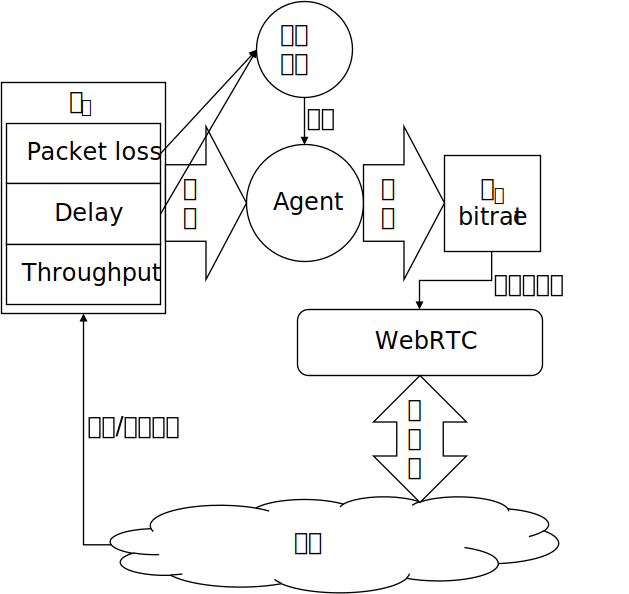
\includegraphics[width=0.9\textwidth, keepaspectratio]{figure/env.pdf}\\
	\caption{智能Agent的任务环境}\label{figure:env}
\end{figure}

\subsection{Agent输入分析}

网络情况所涵盖的变量很多,但大部分变量都记录在路由器、交换机等运营商侧的设备中。显然,实际情况下,运营商不可能在机房中大面积部署高能耗的人工智能应用,也不大可能将通信设备的状况信息开放给用户获取。因此,在客户端侧,Agent所能获取到的信息是比较有限的。根据目前交互式视频通信常用的传输/应用层协议 —— WebRTC的内容,Agent可以通过协议中周期性的RTCP ACK消息收集到每个数据包的发送情况,继而计算出如下的网络状况信息:

\begin{enumerate}[label=\arabic*、]
	\item 丢包率(Packet loss)$l_t$:根据TCP协议中的超时重传规则,在TCP协议中对正常发送的包和重传包进行计数,即获取一定时间内的丢包率信息;
	\item 延迟(Delay)$d_t$:根据TCP协议的ACK机制,对包发送完成和收到确认ACK的时间间隔进行计数,即可获得发送过程的延迟信息;
	\item 吞吐量(Throughput)$t_t$:根据TCP协议中的发送机制,统计一定时间内的发送窗口和接收窗口大小,即可获得系统的吞吐量信息。
\end{enumerate}

令$S_t=(l_t, d_t, t_t)$表示第$t$个计时区间内Agent输入的网络状况信息。

\subsection{Agent输出分析}

由于视频流需要连续发送的特点,在设计Agent时可以不必考虑包发送的时刻问题,而只用考虑一段时间内发送包的数据总量,即视频流的比特率。目前视频流应用常用的WebRTC框架即具有动态调节视频比特率的功能。

在WebRTC框架的每个RTCP循环中,Agent有机会修改下一个循环中的视频编解码器的目标输出比特率。因此,Agent可以将$S_t$映射到一个可选比特率集合$A$(例如$\{0.1Mbps,0.2Mbps,...,2.5Mbps\}$)。经过一段时间的视频传输后,系统又能收集到一批新的网络状况信息,计算出新的状态$S_{t+1}$,进而让Agent生成新的$a_{t+1}$。通过这样的连续迭代,Agent就能学会应对网络动态变化。

\subsection{Agent优化目标分析}\label{sec:Agent优化目标分析}

根据TCP/IP协议的丢包规则,当网络发生拥塞时,数据包在设备中的排队时间将显著增大,网络中无法承载的数据包将被网络设备直接舍弃,在客户端一侧的表现就是丢包率和延迟的急剧增大。因此,如果Agent输出比特率$a_t$超过可用带宽,则将导致网络拥塞,进而在下一个状态$S_{t+1}$中出现较高的丢包率和较大的延迟。因此,通过观察从$S_t$到$S_{t+1}$的丢包率和延迟变化,就能判定网络是否出现拥塞,进而判定Agent输出的$a_t$是否合适。如果$a_t$超过可用带宽,那么当下次观察$S_t$或类似状态时,Agent应输出较小的$a_t$;反之,Agent应输出较大的$a_t$。由此,Agent可以逐步逼近恰好使网路不发生拥塞的视频流比特率。

\section{智能Agent结构}

\subsection{Agent选型}

根据第\ref{sec:任务环境分析}节的分析,直观上讲,本系统所需要的Agent就是一个简单的输入三个变量$(l_t, d_t, t_t)$,输出一个变量$a_t$的函数。但也可以看出,在Agent的运行环境中输出变量$a_t$的取值会反过来影响$t+1$时刻的网络状况;更进一步,Agent的优化目标也是从网络状况$S_t$中计算得到。综上所述,这是一个典型的强化学习模型的运行环境\cite{russell2002artificial},可以使用强化学习模型进行求解。因此,本文将以强化学习模型为核心,介绍在实时交互式视频通信场景下的Agent设计。

\subsection{Agent运行过程}

由第\ref{sec:任务环境分析}节的分析可知,Agent的输入信息均为一段时间内的统计数据,输出也是接下来一段时间内的控制信息,因此输入和输出必然是在一个个时间片上进行的;而用于实时交互式视频传输的流量调节又要求Agent能细粒度地响应网络动态。通常来讲,具有动态调节比特率的视频视频编码器对视频质量的调节粒度均在帧级,即每一帧对应一种比特率,帧与帧之间的比特率可以不同。因此,对于用于实时交互式视频传输的流量调节的Agent,其响应网络动态的粒度极限即是帧级,对应于数十毫秒的时间范围。进而可以得到Agent的运行过程:

\begin{enumerate}[label=\arabic*、]
	\item 初始化:随机选一个较小值作为初始帧的比特率$a_0$;
	\item 传输帧:以比特率$a_{t-1}$对帧进行编码后发送;
	\item 统计$S_t$:在发送帧的过程中,系统收集每个数据包的活动(发送时刻、收到确认ACK的时刻、是否丢包等);
	\item 计算$S_t$:根据统计得到的数据包的活动信息计算出在发送这一帧过程中的平均丢包率、平均延迟和平均吞吐量,作为$(l_t, d_t, t_t)$;
	\item 计算$a_t$:Agent接收$S_t$,计算出下一帧的比特率$a_t$;
	\item 回到第2步,循环。
\end{enumerate}

\subsection{Agent奖励函数}

根据第\ref{sec:Agent优化目标分析}节的分析,在Agent的运行环境中,Agent需要控制WebRTC视频流的比特率实现最高的比特率且使得系统恰好不发生拥塞。因此,根据第\ref{sec:Agent优化目标分析}节的判定方法,Agent的奖励函数要能让系统产生最大的吞吐量以及最小的丢包率和延迟,因此易得奖励函数:

$$r_t=r(a_t)=-\alpha\times l_{t+1}-\beta\times d_{t+1}+\gamma\times t_{t+1}$$

其中$r_t$表示第$t$个时间段内产生的输出$a_t$应用于$t+1$后所产生的奖励;$\alpha$、$\beta$和$\gamma$是训练前需要调节的超参数,表征网络情况的不同方面对系统的影响程度。

\subsection{神经网络结构}

给出适合的Agent结构,及具体模块的结构;
\section{问题}
\begin{enumerate}[label=\arabic*、]
	\item 如何适应动态的网络条件
	\item 大量的Agent在各自的硬件上独立地运行,如何进行训练
	\item 视频编解码器的调节具有滞后性
	\item 掌握机器学习分类算法的性能提升方法;
	\item 能编程实现一些机器学习分类算法并进行性能分析和改进;
	\item 了解人工智能和分类算法的新进展、新应用。
\end{enumerate}
\section{现状}
上述问题的已有解决方法及其优缺点分析;
在虚拟环境中训练
\section{技术分析}
给出采用一个课本中现成方法和算法的优缺点分析,结合上述优缺点分析,进一步给出本文的具体技术和算法方案;
\section{方案分析}
给出本文方案实际应用中的可行性分析。
\bibliography{ref}
\end{document}